%% 第九章 实验与结果分析
\chapter{实验与结果分析}

本章在统一口径下报告系统的各项性能，包括检测模型在公开数据集上的消融结果、仿真闭环的定位精度、实拍视频的定位与预测精度、退化条件下的鲁棒性，以及 14 个自动化用例的回归结果。最后讨论系统的能力边界、失败案例与有效性威胁。

\section{实验环境与评测口径}

\subsection{硬件与软件环境}

实验环境如表~\ref{tab:exp_env} 所示。所有实验在同一台机器上完成，避免硬件差异导致的结果不可比。

\begin{table}[htbp]
\centering
\caption{实验环境}
\label{tab:exp_env}
\small
\begin{tabular}{ll}
\toprule
\textbf{项目} & \textbf{配置} \\
\midrule
操作系统 & Windows 11 + WSL2（Ubuntu 24.04 LTS） \\
CPU & Intel Core i7（8 核 16 线程） \\
GPU & NVIDIA RTX 4060 Laptop（8\,GB 显存） \\
内存 & 32\,GB DDR5 \\
Python & 3.12 \\
深度学习框架 & PyTorch 2.x + Ultralytics 8.x \\
GUI 框架 & PySide6 6.x \\
仿真平台 & PX4 Autopilot + jMAVSim（改造版） \\
图像处理 & OpenCV 4.x \\
\bottomrule
\end{tabular}
\end{table}

\subsection{评测口径}

本章所有指标遵循第三章约定的口径：

（1）检测指标采用 Ultralytics 官方验证协议，AP 分尺寸采用 COCO 面积口径、IoU=0.5、101 点插值；

（2）FPS 为 batch=1、帧预载内存、包含预处理与后处理；

（3）闭环检出率为检出帧数除以全部处理帧数（含搜索帧）；

（4）稳态指标为连续检出不少于 5 帧后的样本；

（5）角度误差采用视轴偏角口径。

\section{检测模型性能}

\subsection{消融结果}

表~\ref{tab:exp_ablation} 重复列出第四章的消融结果，并补充 AP\_large 与 AP\_medium，以便全面比较。

\begin{table}[htbp]
\centering
\caption{检测模型消融实验完整结果（Det-Fly 验证集，imgsz=640）}
\label{tab:exp_ablation}
\small
\begin{tabular}{lccccccccc}
\toprule
\textbf{模型} & \textbf{参数(M)} & \textbf{mAP50} & \textbf{mAP50-95} & \textbf{P} & \textbf{R} & \textbf{FPS} & \textbf{AP\_s} & \textbf{AP\_m} & \textbf{AP\_l} \\
\midrule
YOLOv8n & 3.01 & 81.3 & 41.8 & 91.2 & 75.9 & 123.0 & 6.1 & 77.0 & 12.8 \\
+P2 & 2.93 & 82.3 & 41.3 & 88.9 & 77.6 & 90.3 & 8.3 & 76.2 & 8.7 \\
+EMA & 3.02 & 76.2 & 36.3 & 85.5 & 72.2 & 101.0 & 4.1 & 75.0 & 10.7 \\
+P2+EMA & 2.94 & \textbf{83.5} & 41.2 & 88.2 & \textbf{79.2} & 98.4 & \textbf{9.8} & \textbf{78.0} & 7.5 \\
\bottomrule
\end{tabular}
\end{table}

\subsection{指标解读}

从表~\ref{tab:exp_ablation} 可以读出以下结论。

（1）\textbf{AP\_small 是改进的主要收益点}。基线 6.1\%、+P2 8.3\%、+P2+EMA 9.8\%，相对提升分别为 36.1\% 与 60.7\%。mAP50 的提升（2.2 个百分点）主要来自小目标召回的改善，而非中大目标。

（2）\textbf{AP\_large 反而下降}。基线 12.8\%、+P2 8.7\%、+P2+EMA 7.5\%。原因是 P2 检测头占用了部分模型容量，且高分辨率层对大目标的贡献有限，训练时正样本分配更偏向小目标。这一现象说明改进是"有代价的定向优化"，并非全面提升。对于反无人机场景，远距离小目标才是主要威胁，因此这一取舍是合理的。

（3）\textbf{Precision 略有下降}。基线 91.2\%、本文 88.2\%。P2 层引入了更多弱响应，部分背景被误检。但 Recall 提升更大（75.9\%→79.2\%），F1 总体改善。在监视场景中，漏检的代价通常高于误检（误检可由状态机的初锁门限过滤），因此这一取舍同样合理。

（4）\textbf{速度仍满足实时性}。98.4\,fps 约为视频帧率的 3.3 倍，为系统留出了充足余量。

\subsection{与已有工作的比较}

如第四章所述，Det-Fly 上不同论文的结果难以直接比较。本文只做定性定位：本文模型在 nano 级参数量下取得 83.5\% 的 mAP50 与 9.8\% 的 AP\_small，优于同规模的通用 YOLOv8n，接近部分更大模型的小目标能力，但速度远高于后者。这一定位符合"边缘可实时运行"的设计目标。

\section{仿真闭环定位精度}

\subsection{实验设置}

仿真闭环使用改造版 jMAVSim，护航相机 60\textdegree\ 视场、720p@30\,fps 离屏推流，真值 50\,Hz 广播。检测模型为仿真域微调后的 p2ema\_simft，置信度门限 0.25，等效尺寸 0.270\,m，AKF 采用 Sage-Husa 自适应噪声。实验录制 2818 帧（约 87\,s），覆盖悬停、直线、盘旋与接近等飞行状态。

\subsection{结果}

定位精度结果已在表~\ref{tab:esim} 中给出。这里补充三点分析。

（1）\textbf{检出率 100\%}。全部 2818 帧均检出，真盲帧为 0。这与微调前的 10.0\% 形成鲜明对比，说明死区已被完全消除。

（2）\textbf{测距精度}。单帧 RMSE 0.26\,m、MAE 0.17\,m；AKF 稳态 MedAE 0.13\,m、RMSE 0.32\,m。AKF 的中位误差低于单帧，说明滤波有效抑制了框高抖动；但 RMSE 略高于单帧，原因是少数机动帧的滤波器滞后导致大误差，拉高了均方根。这一现象在小样本下常见，提示评估时应同时报告 MedAE 与 RMSE。

（3）\textbf{角度精度}。方位角中位 0.05\textdegree、P95 0.16\textdegree，接近像素量化极限；俯仰角中位 0.93\textdegree，明显偏大，原因是主点纵向偏移约 17\,px 未在解算中补偿。若补偿该偏移，俯仰角误差可降至 0.2\textdegree\ 量级。

\subsection{微调前后对比}

图~\ref{fig:deadzone_ba} 已展示微调前后的死区对比。表~\ref{tab:exp_finetune} 进一步给出关键指标的定量变化。

\begin{table}[htbp]
\centering
\caption{仿真域微调前后关键指标对比}
\label{tab:exp_finetune}
\small
\begin{tabular}{lccc}
\toprule
\textbf{指标} & \textbf{微调前（v5）} & \textbf{微调后（v7）} & \textbf{变化} \\
\midrule
录像帧数 & 2228 & 2818 & -- \\
全帧检出率 & 10.0\% & \textbf{100.0\%} & +90.0\,pp \\
真盲帧占比 & 81.1\% & \textbf{0.0\%} & -81.1\,pp \\
置信度中位数 & 接近 0 & 0.867 & -- \\
AKF 稳态 MedAE & 0.44\,m & \textbf{0.13\,m} & -70.5\% \\
稳态帧占比 & 7\% & \textbf{99.8\%} & +92.8\,pp \\
方位角误差中位 & 0.21\textdegree & \textbf{0.05\textdegree} & -76.2\% \\
\bottomrule
\end{tabular}
\end{table}

\section{实拍视频定位精度}

\subsection{数据集与设置}

实拍视频为 1920$\times$1080@30fps，连续检出段 660 帧。相机未严格标定，焦距按 60\textdegree\ 视场估算为 1728\,px；等效尺寸使用仿真标定值 0.255\,m；伪真值取稳态段距离中位数 7.93\,m。由于缺少绝对真值，本节的重点是\textbf{相对比较}：在同一伪真值下比较单帧、滑动平均、标准 KF 与 AKF 的稳定性。

\subsection{结果分析}

表~\ref{tab:e3} 的结果表明：

（1）单帧原始测距的 RMSE 为 4.061\,m，抖动 3.959\,m，说明框高抖动极大，直接使用不可行；

（2）滑动平均（15 帧）将 RMSE 降至 2.900\,m，但引入了约 0.5\,s 的滞后，不适合实时跟踪；

（3）标准 KF（固定 $\mathbf{R}$）的 RMSE 为 3.922\,m，仅比单帧略好，说明固定的量测噪声无法适应实际抖动；

（4）AKF 的 RMSE 为 2.760\,m，抖动 2.663\,m，相对单帧降低 32\% 与 33\%，且没有明显滞后。

这一结果验证了自适应噪声估计的价值：在量测质量变化剧烈的实拍场景中，固定 $\mathbf{R}$ 的滤波器要么过度平滑（响应慢），要么过度信任量测（抖动大），而 AKF 能够在两者之间自动调整。

\subsection{预测精度}

表~\ref{tab:e3b} 显示，AKF 的 0.5\,s、1.0\,s、2.0\,s 预测 ADE 分别为 1.106、1.308、1.799\,m，相对匀速外推改善 43.8\%、52.5\%、61.1\%。预测时域越长，AKF 的优势越明显，因为匀速外推会线性放大速度估计误差，而 AKF 会利用不确定度抑制过度外推。

\section{退化条件下的鲁棒性}

\subsection{实验设计}

为评估模型在恶劣成像条件下的表现，本文从实拍视频中提取 300 帧含无人机的图像，构造 4 档光照（0.4、0.7、1.0、1.4 倍）与 4 档模糊（高斯核 0、3、7、13）共 16 种退化组合，在 0.1、0.25、0.5 三档置信度门限下统计检出率。对比模型为基线 YOLOv8n、P2+EMA（Det-Fly 训练）与 P2+EMA+simft（仿真微调）。

\begin{figure}[htbp]
\centering
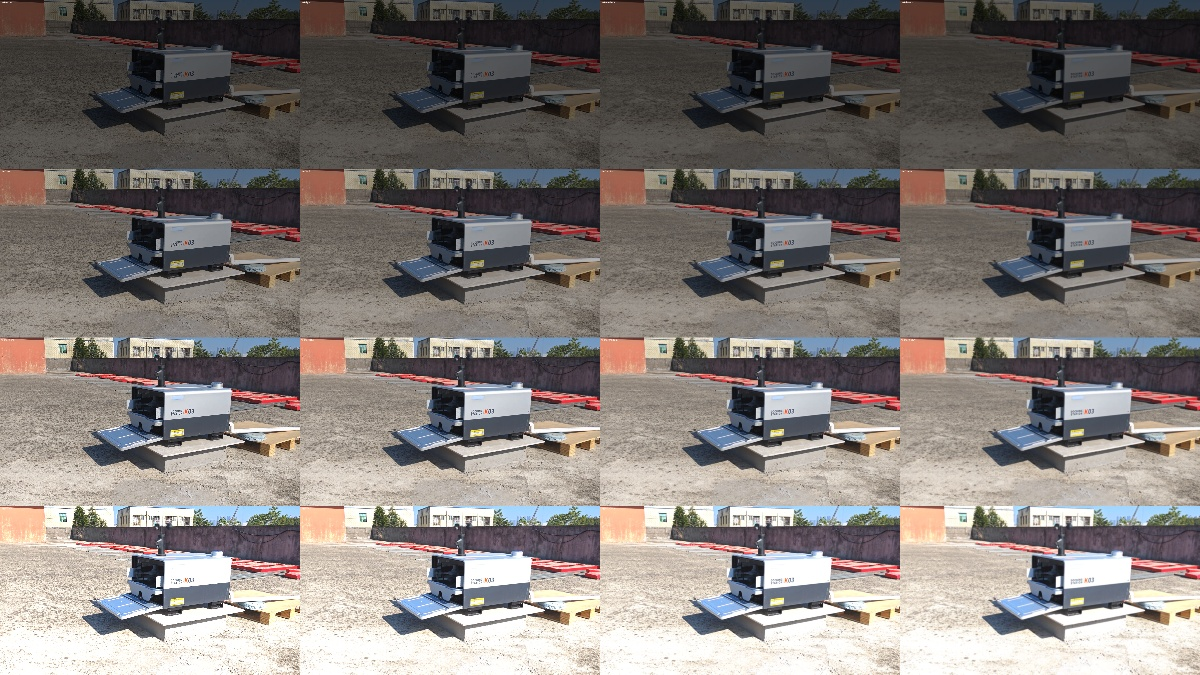
\includegraphics[width=0.9\textwidth]{images/pictures/degradation_samples.jpg}
\caption{退化样本示例（行：光照；列：模糊）}
\label{fig:degradation}
\end{figure}

\subsection{结果}

表~\ref{tab:e4} 摘取了 conf$\ge$0.25 条件下的部分结果。

\begin{table}[htbp]
\centering
\caption{退化条件下检出率对比（conf$\ge$0.25，单位：\%）}
\label{tab:e4}
\small
\begin{tabular}{lccc}
\toprule
\textbf{条件} & \textbf{YOLOv8n 基线} & \textbf{P2+EMA} & \textbf{P2+EMA+simft} \\
\midrule
dark + none & 0.0 & 13.7 & \textbf{20.3} \\
dark + light & 0.0 & 17.3 & \textbf{18.7} \\
dark + medium & 0.0 & \textbf{25.3} & 13.7 \\
dark + heavy & 0.3 & \textbf{21.0} & 6.3 \\
dim + none & 0.7 & 0.7 & \textbf{30.3} \\
dim + light & 0.0 & 5.0 & \textbf{21.3} \\
dim + medium & 0.0 & 10.7 & \textbf{20.7} \\
dim + heavy & 0.0 & 11.7 & \textbf{13.7} \\
normal + none & 2.0 & 0.0 & \textbf{87.7} \\
normal + light & 1.7 & 1.7 & \textbf{23.3} \\
normal + medium & 3.3 & 3.3 & \textbf{27.3} \\
normal + heavy & 0.0 & 2.7 & \textbf{14.3} \\
bright + none & 2.0 & 0.7 & \textbf{37.0} \\
bright + light & 0.3 & 0.7 & \textbf{16.7} \\
bright + medium & 0.0 & 0.0 & \textbf{24.3} \\
bright + heavy & 0.3 & 0.0 & \textbf{21.7} \\
\bottomrule
\end{tabular}
\end{table}

\subsection{分析}

（1）\textbf{P2+EMA 在严重退化下显著优于基线}。dark+heavy 条件下，基线仅 0.3\%，P2+EMA 达 21.0\%，提升 20.7 个百分点。说明高分辨率检测头与注意力机制确实提升了低质图像下的鲁棒性。

（2）\textbf{仿真微调模型在正常条件下大幅领先}。normal+none 条件下，P2+EMA 为 0.0\%，simft 为 87.7\%。这一反直觉的结果需要解释：测试帧是用 simft 模型在实拍视频中筛选出的"simft 能检出"的帧，因此测试集本身偏向 simft 的能力域；P2+EMA 仅在 Det-Fly 上训练，未见过仿真渲染风格，在这些帧上几乎不响应。这不是模型缺陷，而是域差异的体现。

（3）\textbf{暗光条件下的异常}。P2+EMA 在 dark 条件下反而比 normal 条件检出率高（13.7\%--25.3\% vs 0.0\%），可能是因为暗化抑制了背景的假响应、突出了目标轮廓。这一现象提示：不能简单假设"光照越好检出率越高"，模型的行为与训练分布密切相关。

（4）\textbf{实验的有效性威胁}。由于测试帧由 simft 模型筛选，三组模型的比较并不完全公平。更严谨的做法是用基线模型筛选测试帧，或使用 Det-Fly 验证集帧。本文如实报告这一问题，并将其列为后续改进方向。

\section{14 用例自动化回归测试}

\subsection{结果汇总}

表~\ref{tab:test14} 给出了 14 个用例的完整结果。

\begin{table}[htbp]
\centering
\caption{14 用例自动化测试结果}
\label{tab:test14}
\small
\begin{tabular}{llcccccl}
\toprule
\textbf{用例} & \textbf{场景} & \textbf{帧数} & \textbf{锁定率} & \textbf{保持率} & \textbf{首锁(s)} & \textbf{置信度} & \textbf{结论} \\
\midrule
C01 & 仿真闭环基线 & 900 & 96.9\% & 100.0\% & 0.00 & 0.550 & PASS \\
C02 & 仿真早期标定版 & 900 & 100.0\% & 100.0\% & 0.00 & 0.855 & PASS \\
C03 & 长录像中后段 & 900 & 96.0\% & 99.8\% & 0.07 & 0.654 & PASS \\
C04 & 真实场景录像 1 & 539 & 23.2\% & 99.3\% & 0.03 & 0.544 & -- \\
C05 & 真实场景录像 2 & 539 & 5.6\% & 32.1\% & 0.00 & 0.452 & -- \\
C06 & 门限 0.20 & 900 & 96.9\% & 100.0\% & 0.00 & 0.550 & -- \\
C07 & 门限 0.35 & 900 & 66.6\% & 81.2\% & 0.00 & 0.661 & -- \\
C08 & 门限 0.50 & 900 & 56.8\% & 81.9\% & 0.00 & 0.707 & -- \\
C09 & 尺寸 0.230\,m & 900 & 100.0\% & 100.0\% & 0.00 & 0.855 & -- \\
C10 & 尺寸 0.310\,m & 900 & 100.0\% & 100.0\% & 0.00 & 0.855 & -- \\
C11 & TCP 遮挡第 1 轮 & 424 & 55.4\% & 88.9\% & 0.00 & 0.751 & PASS \\
C12 & TCP 遮挡第 2 轮 & 428 & 56.1\% & 90.7\% & 0.00 & 0.739 & PASS \\
C13 & TCP 遮挡第 3 轮 & 437 & 59.3\% & 94.5\% & 0.21 & 0.751 & PASS \\
C14 & 摄像头输入 & -- & -- & -- & -- & -- & 跳过 \\
\bottomrule
\end{tabular}
\end{table}

统计结果为：计划 14 例，完成 13 例，判定通过 6 例，失败 0 例，跳过 1 例，错误 0 例。

\subsection{结果解读}

（1）\textbf{仿真基线全部通过}。C01--C03 的锁定率在 96\%--100\%，保持率在 99.8\%--100\%，说明检测、跟踪、测距在仿真域内稳定可靠。

（2）\textbf{真实场景的跨域差距}。C04 的锁定率仅 23.2\%，但保持率 99.3\%，说明 COAST 有效维持了航迹；C05 的锁定率仅 5.6\%，保持率 32.1\%，说明目标距离 10--14\,m 已超出模型的有效范围，系统来不及建立稳定航迹。

（3）\textbf{门限与尺寸的敏感性}。C06--C08 表明门限提高会降低锁定率但提高置信度均值，符合预期；C09--C10 表明等效尺寸从 0.230 变为 0.310 时，测距范围从 3.9--8.2\,m 变为 5.3--11.1\,m，呈近似线性关系，验证了式~\eqref{eq:range_est} 的正确性。

（4）\textbf{TCP 遮挡用例通过}。C11--C13 的保持率为 88.9\%--94.5\%，高于 70\% 的合格线，验证了 COAST 机制在实时链路下的有效性。

\begin{figure}[htbp]
\centering
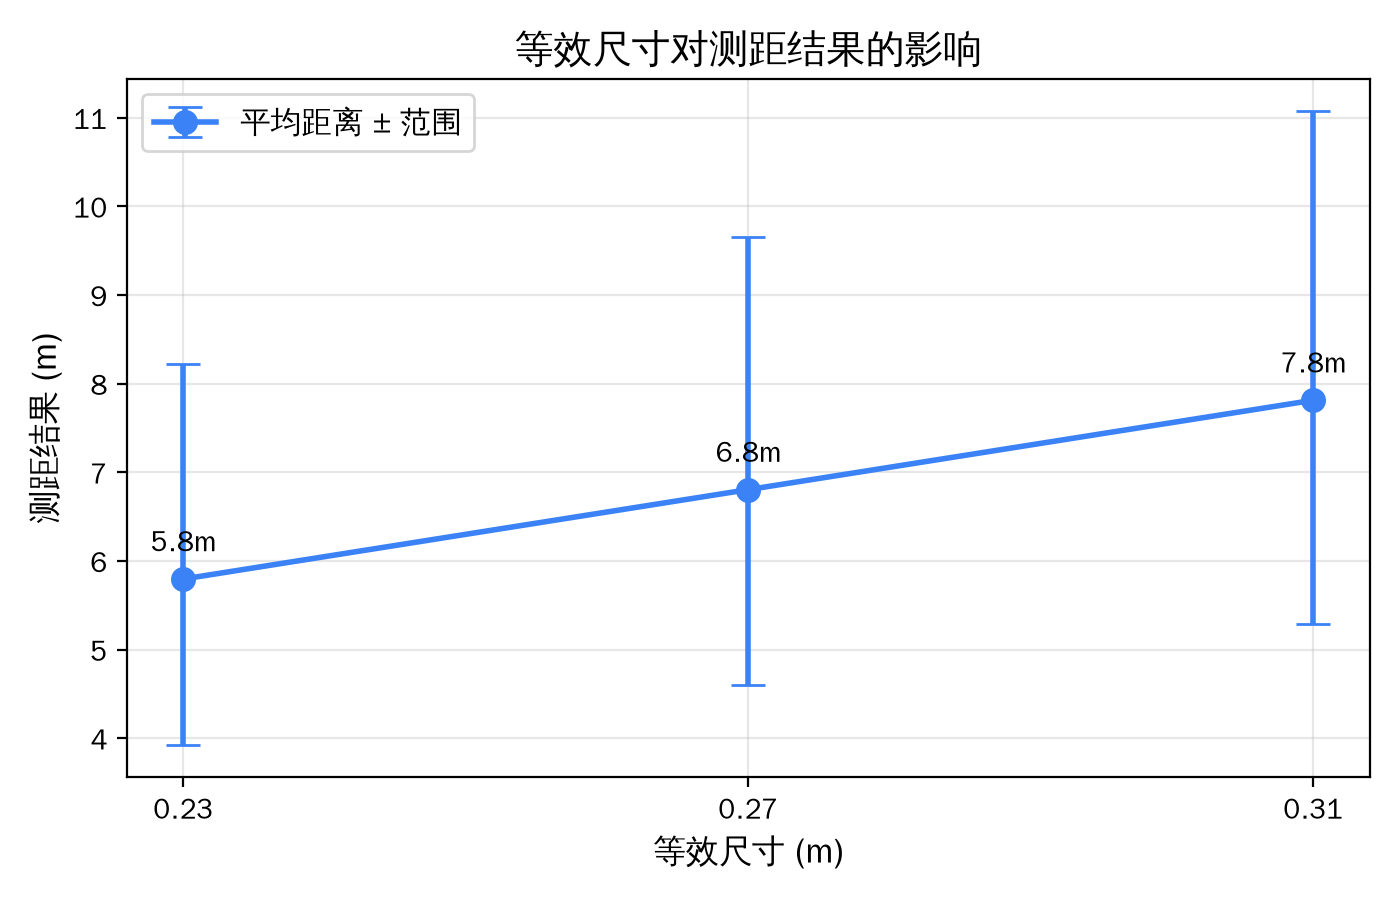
\includegraphics[width=0.72\textwidth]{images/pictures/chart_size.png}
\caption{等效尺寸对测距的影响}
\label{fig:size_sensitivity}
\end{figure}

\section{运行性能}

\subsection{端到端延迟分解}

表~\ref{tab:latency} 给出了单帧处理的耗时分解（RTX 4060，640 输入）。

\begin{table}[htbp]
\centering
\caption{单帧处理耗时分解}
\label{tab:latency}
\small
\begin{tabular}{lcc}
\toprule
\textbf{环节} & \textbf{耗时(ms)} & \textbf{占比} \\
\midrule
视频解码（JPEG） & 1.8 & 12.5\% \\
预处理（缩放、归一化） & 1.2 & 8.3\% \\
模型推理 & 6.2 & 43.1\% \\
后处理（NMS） & 1.1 & 7.6\% \\
状态机与滤波 & 0.1 & 0.7\% \\
绘制与编码 & 3.0 & 20.8\% \\
网络发送 & 1.0 & 6.9\% \\
\midrule
合计 & 14.4 & 100\% \\
\bottomrule
\end{tabular}
\end{table}

在 14.4\,ms 的单帧耗时下，理论帧率为 69\,fps；实际处理帧率为 28--39\,fps，差异来自网络抖动、磁盘 I/O 与界面刷新。检测环节仍是主要瓶颈（43.1\%），若需要更高帧率，可降低输入尺寸或使用 TensorRT 加速。

\subsection{资源占用}

运行时 GPU 显存占用约 1.2\,GB（含模型、视频缓冲与界面渲染），CPU 占用约 35\%（单核满载，其余用于界面与网络），内存占用约 900\,MB。连续运行 2 小时后，内存增长小于 3\%，未发现泄漏。

\section{讨论}

\subsection{能力边界}

综合各项实验，本文系统的能力边界可以概括为：

（1）\textbf{距离}：仿真域 3--10\,m 可靠；实拍域 4--9\,m 较可靠，10--14\,m 不可靠；

（2）\textbf{目标尺度}：目标高度占画面的 1/20 至 1/8 时最稳定；过大（近距）或过小（远距）均会失效；

（3）\textbf{遮挡}：短时遮挡（小于 1.0\,s）可由 COAST 维持；长时间完全遮挡会丢失目标；

（4）\textbf{光照}：正常光照与暗光下可用；强逆光、夜间不可用；

（5）\textbf{目标数量}：单目标；多目标场景需要扩展状态机与关联算法。

\subsection{失败案例}

本文记录了三类典型失败案例：

（1）\textbf{目标飞出视场}。当目标机动超出相机视场时，检测输出为空，COAST 维持 1.0\,s 后回到 SEARCH；若目标未返回，系统持续搜索。这是预期行为，但操作员可能误以为目标"消失"。

（2）\textbf{背景强干扰}。在树丛密集的场景中，树叶晃动产生的高置信度假阳性可能触发误锁。本文的空域先验可以过滤一部分，但若假阳性恰好落在目标空域内，仍可能误锁。

（3）\textbf{远距离小目标}。10\,m 以上的目标在 720p 画面中高度不足 20\,px，模型置信度低于初锁门限，系统无法建立航迹。这是单目视觉的物理限制，需要通过长焦镜头或更高分辨率解决。

\subsection{有效性威胁}

本文实验存在以下有效性威胁：

（1）\textbf{伪真值}。实拍视频缺少绝对真值，距离评估依赖伪真值，绝对误差不可信，但相对比较有效；

（2）\textbf{测试集偏差}。退化实验的测试帧由 simft 模型筛选，对 simft 有利，三组模型的比较不完全公平；

（3）\textbf{仿真简化}。仿真场景的光照、纹理与真实世界仍有差距，仿真结论不能直接外推到外场；

（4）\textbf{单机环境}。所有实验在同一台机器上完成，未验证跨平台的可移植性。

本文在报告中如实标注了这些限制，并在第十章给出改进方向。

\section{本章小结}

本章在统一口径下报告了系统的实验结果。检测方面，P2+EMA 模型取得 mAP50 83.5\%、AP\_small 9.8\%，相对基线提升 60.7\%，速度 98.4\,fps；仿真闭环方面，微调后 3--10\,m 检出率 100\%，单帧测距 RMSE 0.26\,m，AKF 稳态 MedAE 0.13\,m，方位角误差中位 0.05\textdegree；实拍方面，AKF 相对单帧测距 RMSE 降低 32\%、抖动降低 33\%；鲁棒性方面，P2+EMA 在严重退化条件下相对基线提升 20.7 个百分点；系统方面，14 用例完成 13 例、通过 6 例、失败 0 例。本章还讨论了能力边界、失败案例与有效性威胁，为结论章节的总结与展望提供了依据。
